\documentclass[a4paper]{ctexart}
\usepackage{amsmath}
\usepackage{graphicx}
\usepackage{float}

\bibliographystyle{plain}

\title{超市数据分析报告}
\author{}
\date{\today}


\begin{document}
\maketitle
\tableofcontents
\section{项目背景}
自 2015 年 Q1 至 2018 年 Q4 零售行业主要呈现三大趋势:
\begin{itemize}
    \item 线上线下融合加速落地。就表现形式而言,主要由基于消费体验重构的融合、供应链效
          率提升与渠道下沉以及消费场景延伸是线上线下融合的三类形式。
    \item 社交电商异军突起。模式上主要分为现有流量入口的商业价值挖掘和平台化运营两大
          类。
    \item 泛零售品类不断扩展。横向扩充与纵向延伸同步推进。 此外,从消费端趋势来看,以
          代际变迁与消费升级为核心的基本趋势将长期持续存在。
          本报告是基于该大环境为载体的,分析办公相关某商超领域的数据表现。
\end{itemize}


\section{数据获取}
现有 \emph{9959} 条超市数据,其中
$\text{利润率} = \text{销售额}/\text{利润}$
$(\cdot)$表示负值。


\section{数据模型选定}
维度:地区、城市、订单日期、类别和子类别等;
度量:产品类别、销售额、利润和订单量等;
度量和相应的维度关系如图~\ref{fig:mindmap}所示。
\begin{figure}[H]
    \centering
    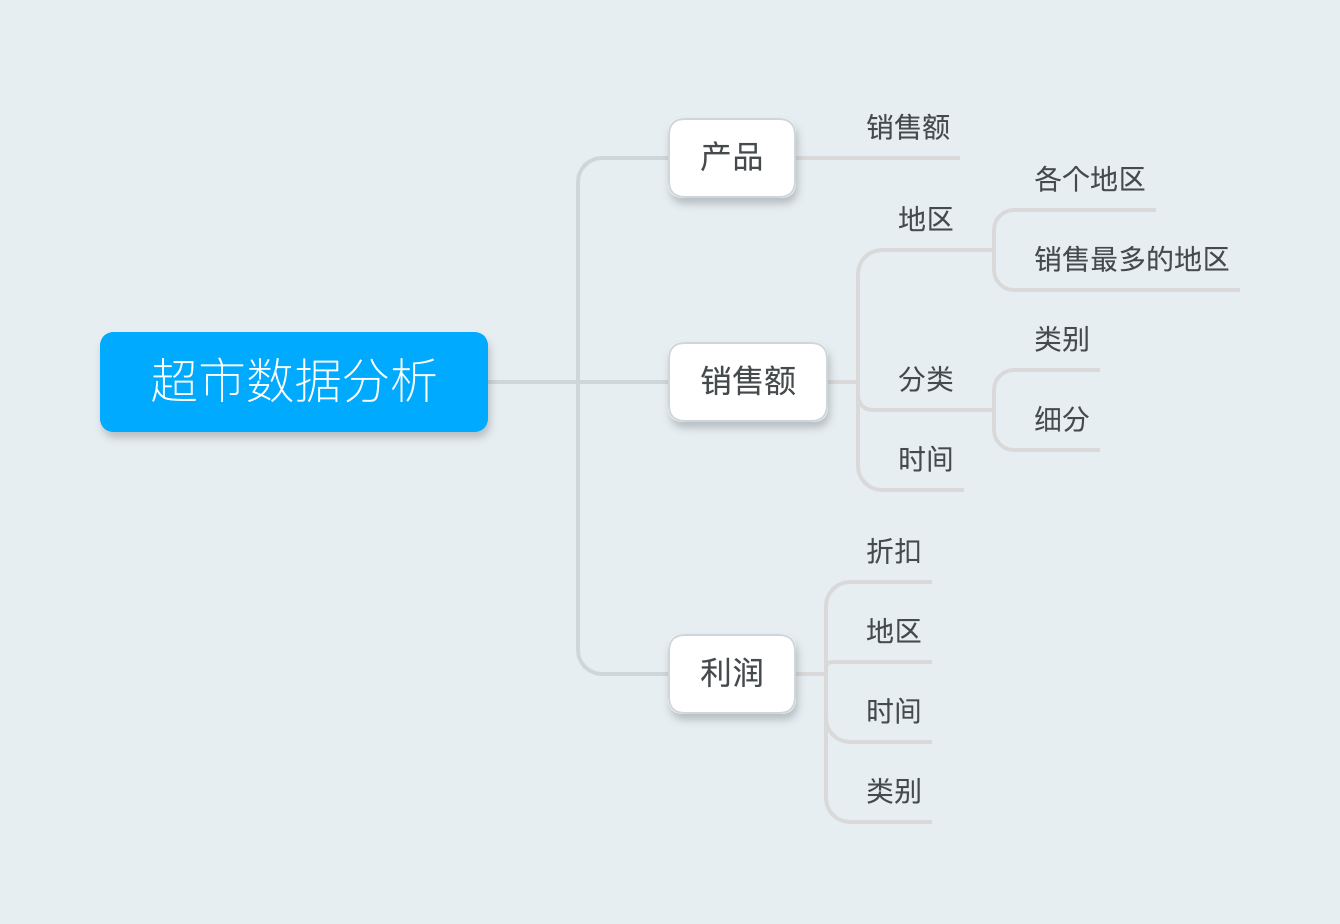
\includegraphics[width=\textwidth]{figures/mindmap}
    \caption{度量和相应的维度关系}\label{fig:mindmap}
\end{figure}
\newpage
\subsection{产品类别}
    根据产品的不同类别分析其平均销售量。
\subsection{销售额}
\begin{enumerate}
    \item 分析各个地区的销售额分布图,根据销售额最多的地区看城市分布,观测是
          否与认知中城市 GDP 及产能相对应与匹配;
    \item 根据各个类别的商品进行销售额分析,再细分至公司与个人,观测采购的类
          别商品与该区域的公司分布与人群有怎样的线性关系;
    \item 按照时间维度去看销售额分布情况,对照客观存在活动内容及运营数据反观
          数据表现;
\end{enumerate}
\subsection{利润}
\begin{enumerate}
    \item 通过不同的地区与时间,结合折扣情况,看利润的数据表现;
    \item 通过不同的类别,看利润分布情况;
\end{enumerate}

\section{数据整理}
将数据进行格式调整,本次处理主要针对带有括号或货币符号的数值进行处理;


\section{描述分析}
\subsection{各产品类别与销售额的关系}
\begin{figure}[H]
    \centering
    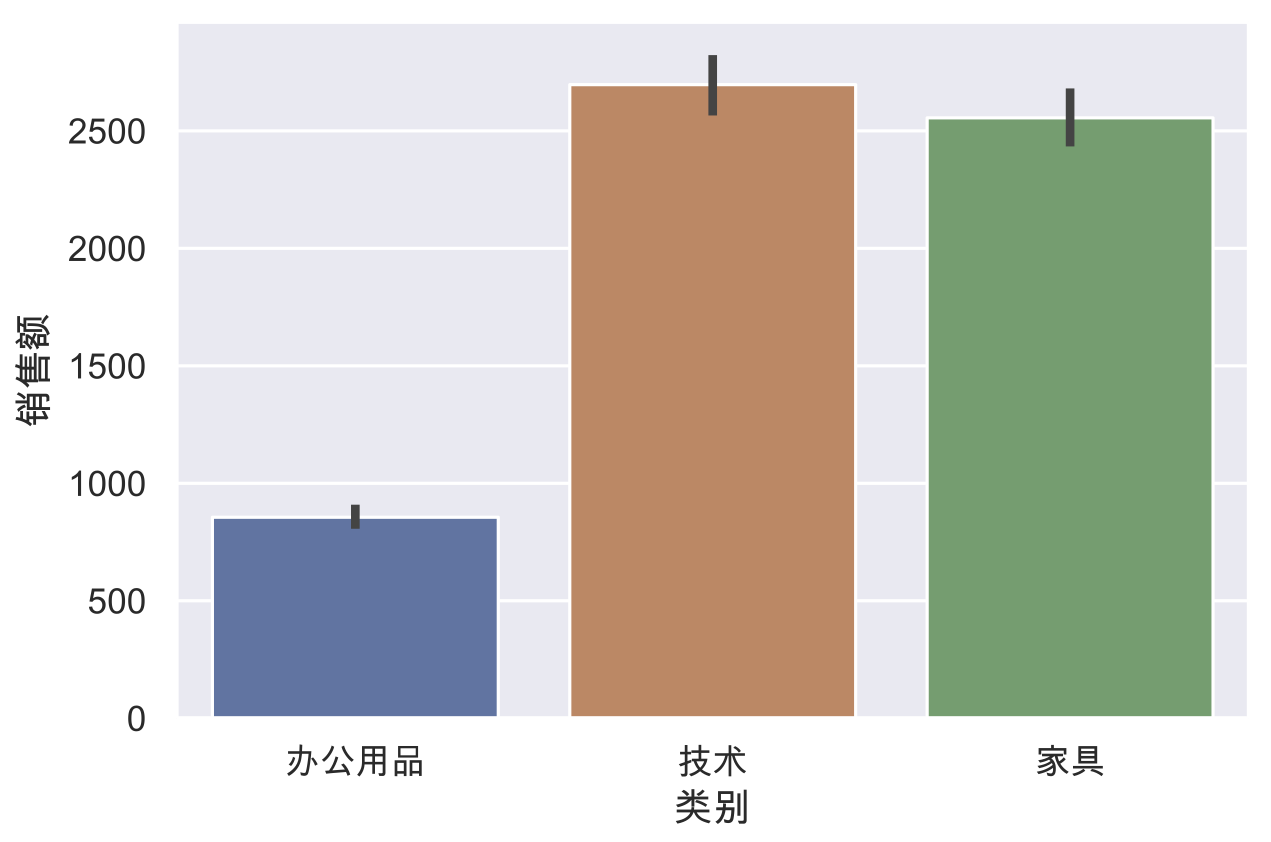
\includegraphics[width=.7\textwidth]{figures/prod_avg}
    \caption{各产品类别的销售额}\label{fig:prod}
\end{figure}
从图~\ref{fig:prod}中可以看出,不同类别的产品销售额的平均值是不一样的。其中,技术类产品最高,而办公用品类最低。

\subsection{销售额按照地区与细分消费划分}
\begin{figure}[H]
    \centering
    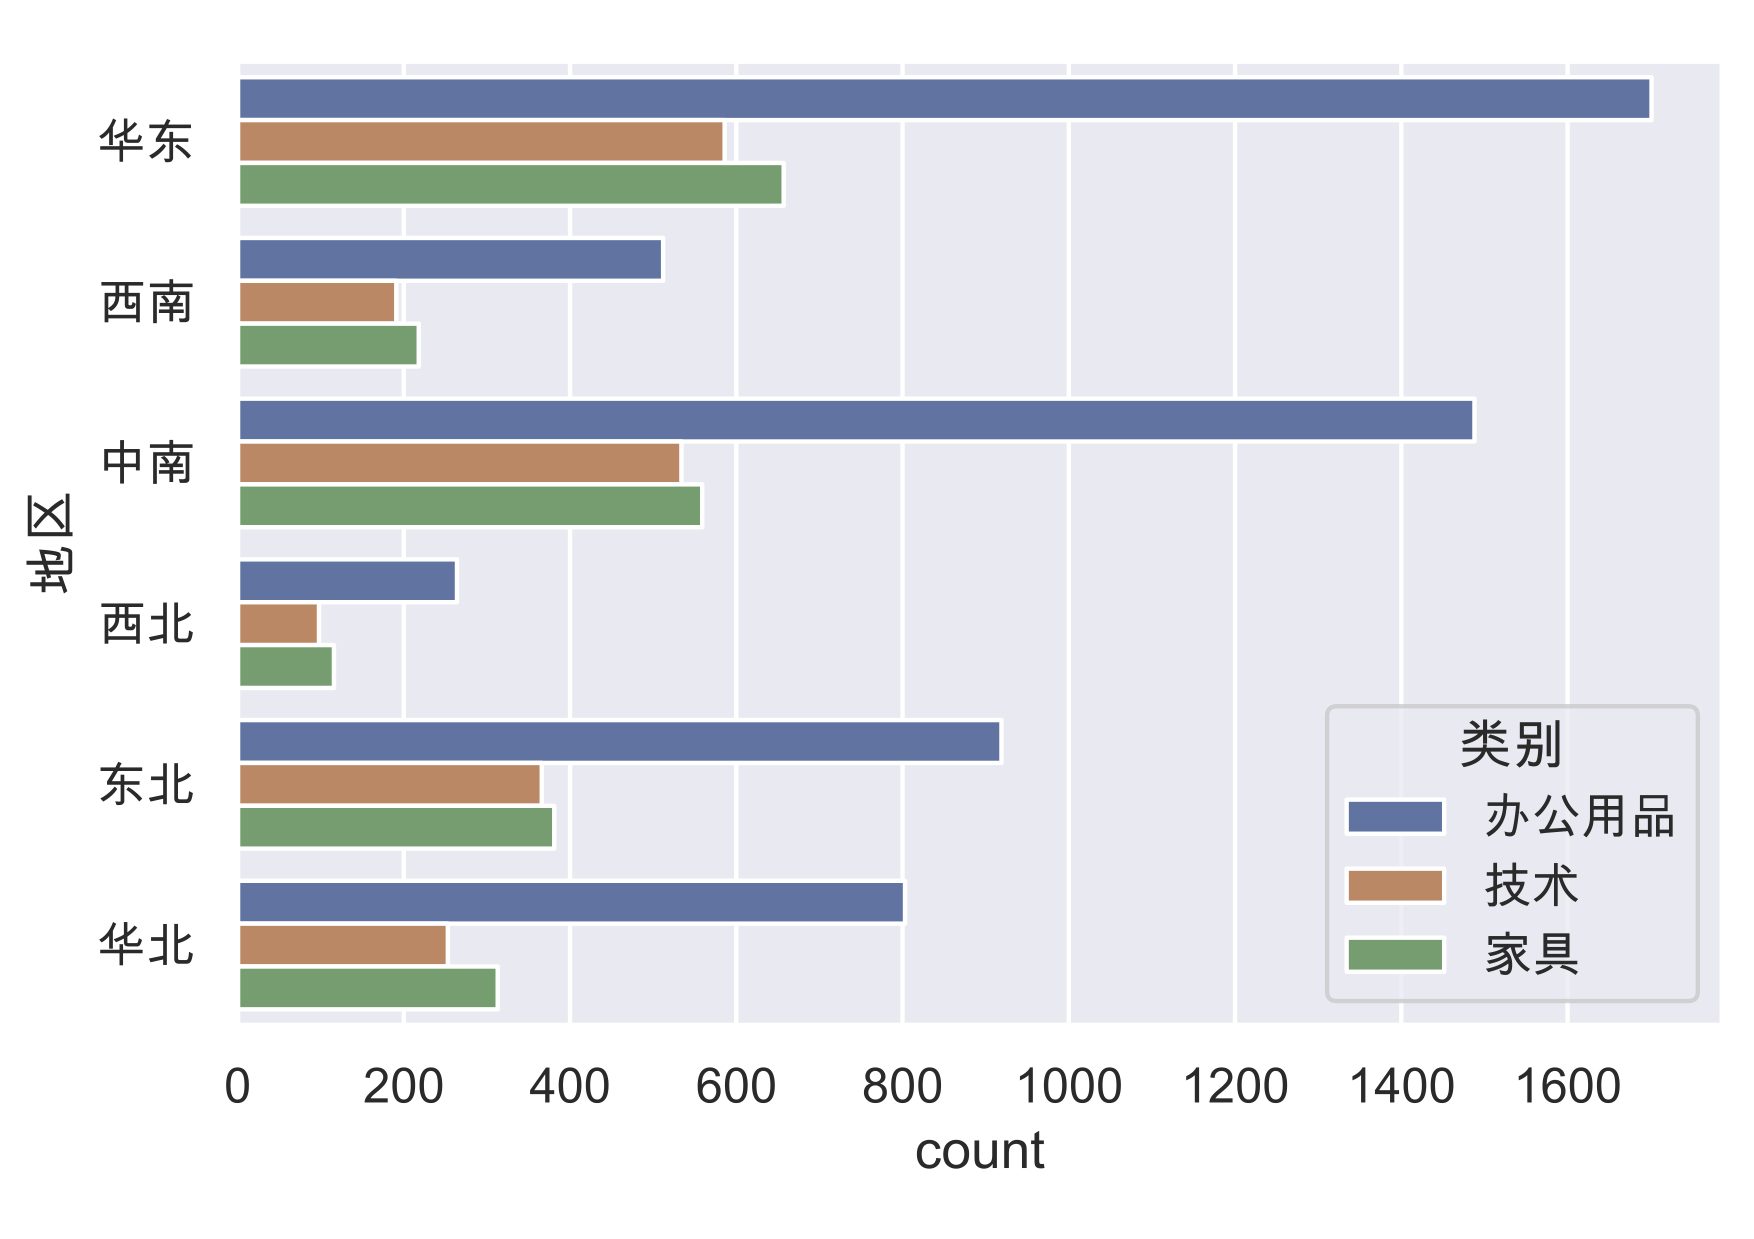
\includegraphics[width=\textwidth]{figures/area_count}
    \caption{各地区不同产品类别的订单量}
\end{figure}
该超市的消费区域来看,华东地区的订单量最多,在各个地区中,办公用品占比最大。

\begin{figure}[H]
    \centering
    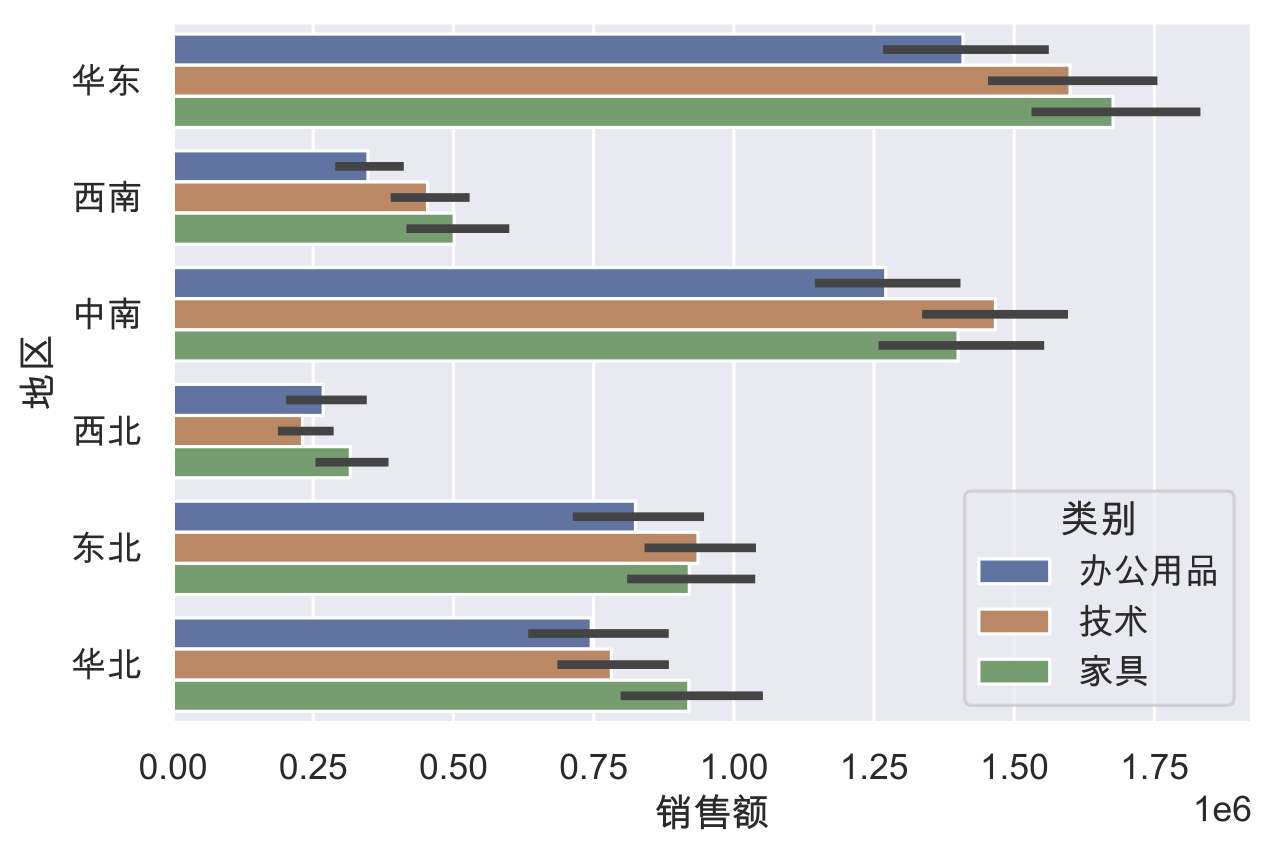
\includegraphics[width=\textwidth]{figures/area_total}
    \caption{各地区不同产品类别的销售额}
\end{figure}
类似地,华东地区的销售额最多,在各个地区中,办公用品占比最大。


\begin{figure}[H]
    \centering
    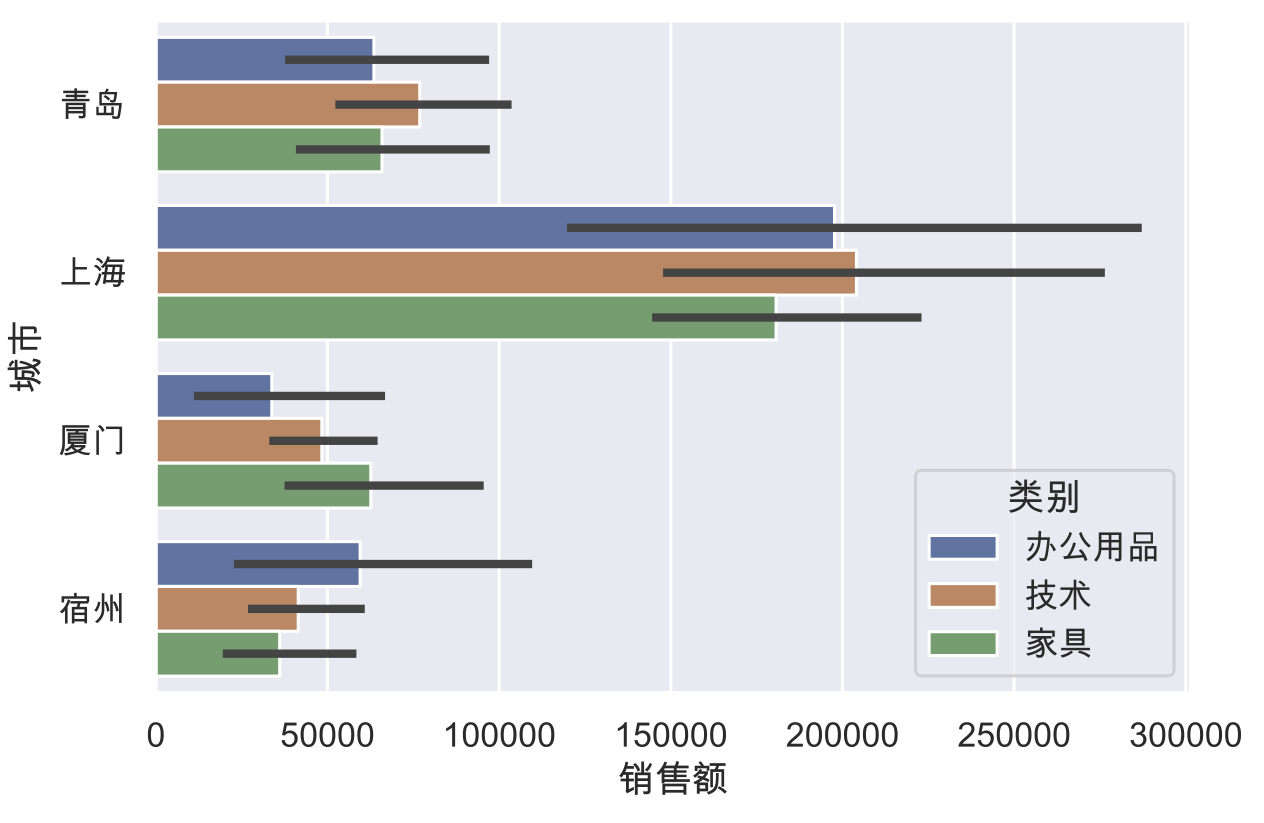
\includegraphics[width=\textwidth]{figures/city_total}
    \caption{华东地区销售额前4城市不同产品类别的销售额}
\end{figure}
继续细分华东区销售额分布,其中四个城市的销售额数据表现较为突出


\subsection{销售额与利润的关系}
\begin{figure}[H]
    \centering
    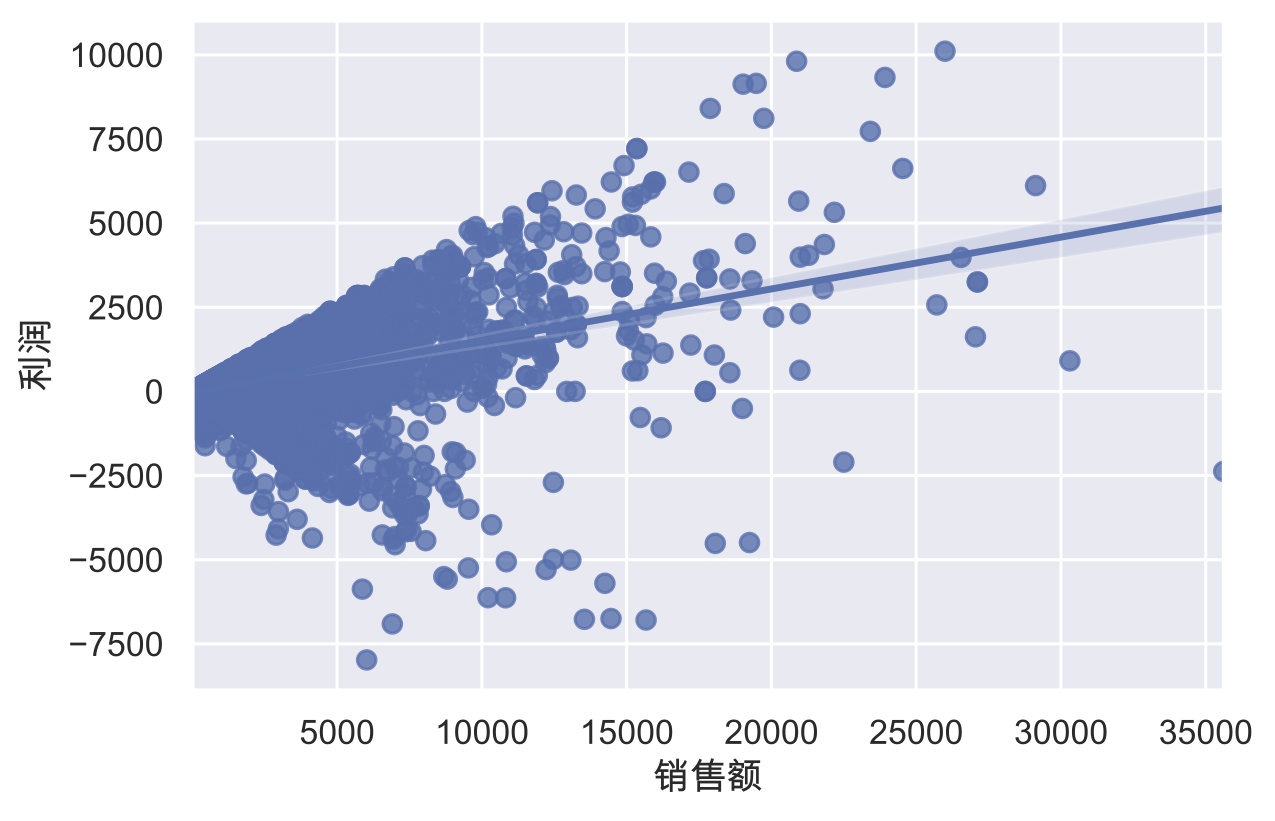
\includegraphics[width=\textwidth]{figures/rel}
    \caption{销售额与利润的关系}
\end{figure}
销售额和利润在被产品名称细分的情况下,呈现非常明显的线性关系($p$ 值< 0.01)。

\subsection{利润与地区的关系}
\begin{figure}[H]
    \centering
    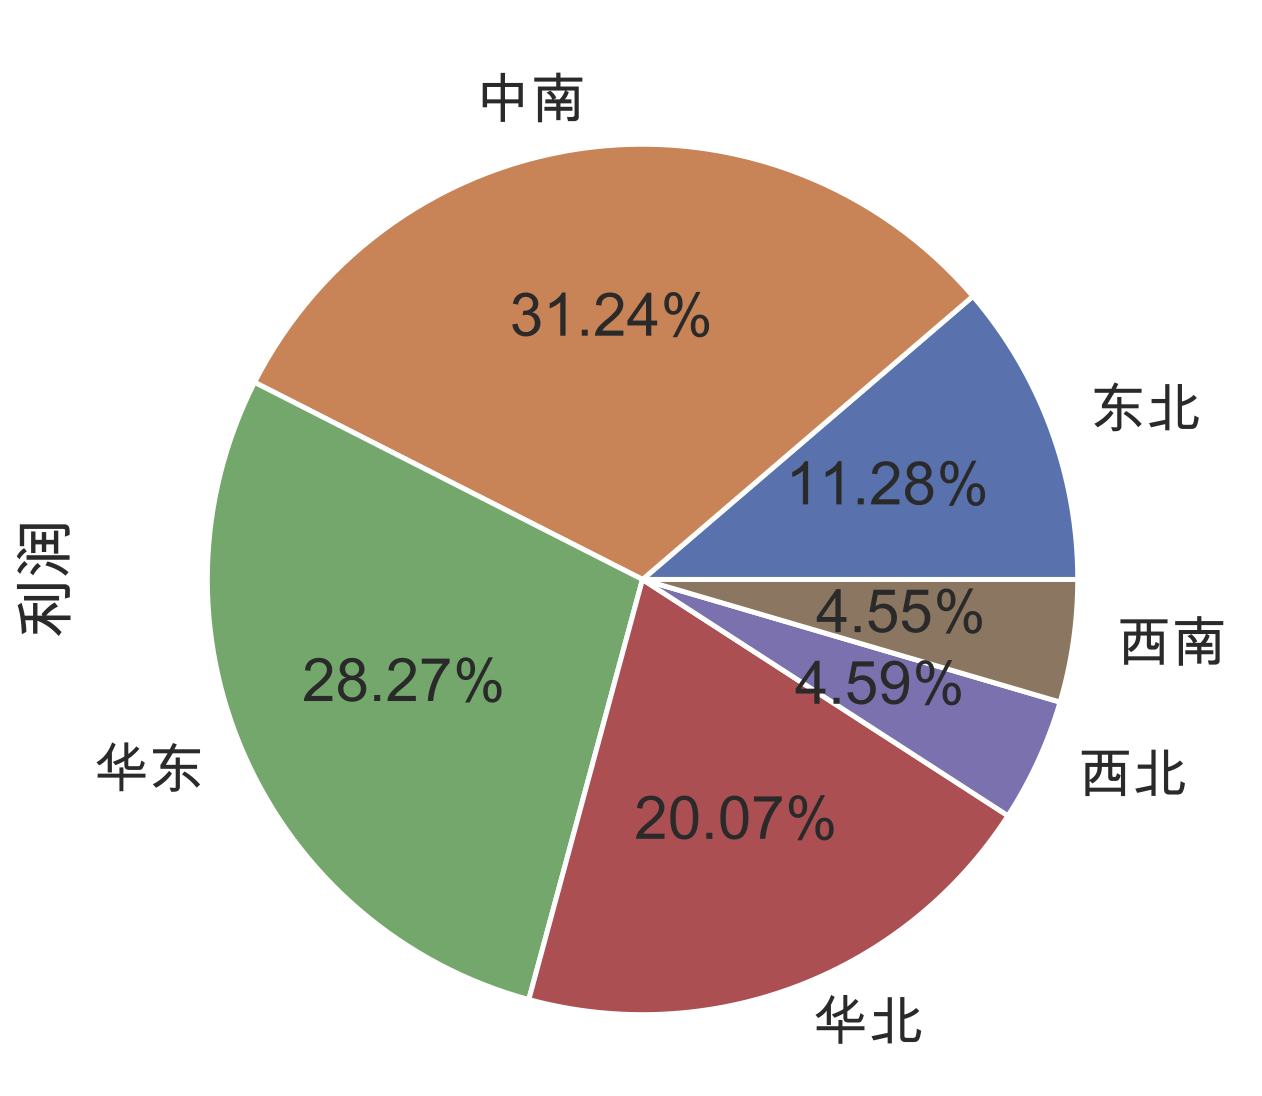
\includegraphics[width=.5\textwidth]{figures/pie}
    \caption{各地区的利润占比}
\end{figure}
地区为中南的利润最多,中南、华东、华北所占的比重超过了 66.66\%,达到了
77.31\%。可见,即使销售额与利润成明显的线性关系,但利润在不同地区还是呈现了
稍有不同的数据表现。

\subsection{各类别产品利润分布情况}
\begin{figure}[H]
    \centering
    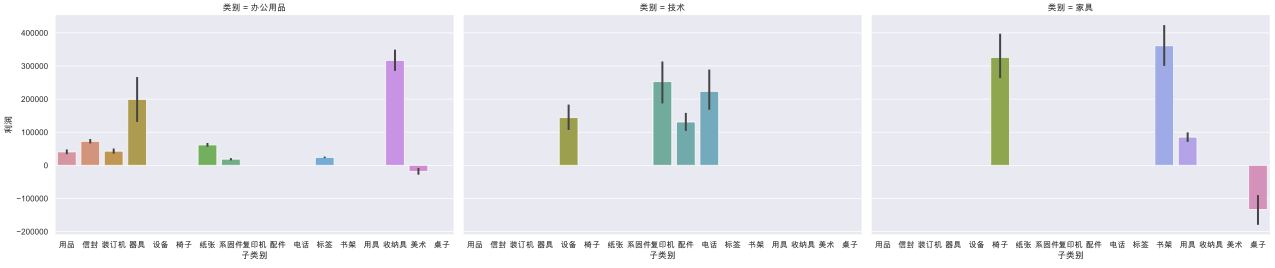
\includegraphics[width=1.2\textwidth]{figures/prod_cat}
    \caption{各类别产品的利润分布}
\end{figure}
由图可见,三大类产品,办公用品利润最高,其中收纳具的利润最高,远高于其他品类,
但其中美术的利润较低,家具与技术类的产品数据表现基本相似,但家具类桌子的利润相对
较低。

\subsection{订单日期及销售额}
\begin{figure}[H]
    \centering
    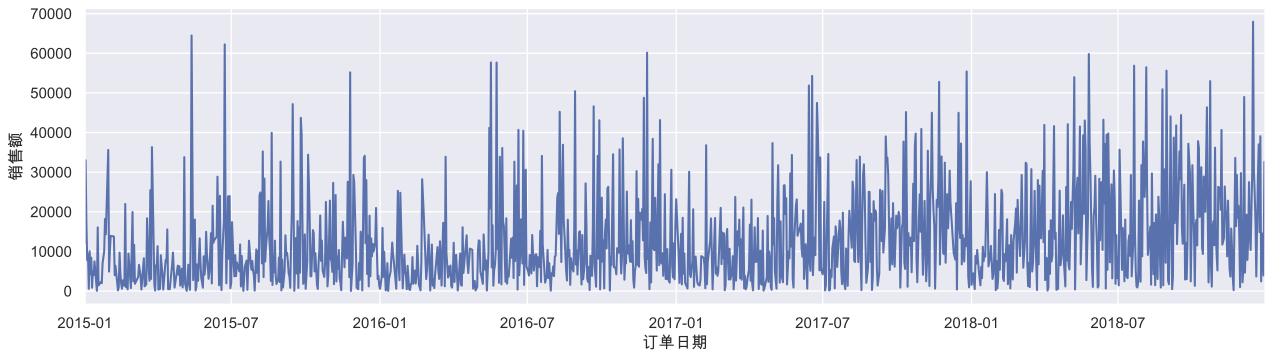
\includegraphics[width=1.2\textwidth]{figures/time}
    
    \caption{销售额与日期的关系}
\end{figure}
由订单分布图可见,自 2015 年至 2018 年,每年 6 月与 11 月销售额将处于一个
次波峰与波峰,其他时间,动态波动;
\newpage


\section{总结}
结合本次样本(办公相关产品在 2015 年~2018 年数据)数据表现整体呈稳步上升
趋势,结合国家的政策来看,在 2014 下半年发布的鼓励“大众创业,万众创新”,以长
江三角洲为发射点的创业之光直接映射到各领域、地区。

在未来,我认为地区地区间消费日趋均衡,高质量发展是方向,一方面, 由于网络零售和零售赋能带来的普惠效应,
消费市场的地域鸿沟得以逐渐弥合(在消费数量和品质方面均有体现) ;另一方面,在行
业端与消费端的共同驱动下,消费品质与服务体验得以持续提升,朝着高质量发展的方
向前进。

\bibliography{bibdata/refs}
\nocite{*}

\end{document}
